\documentclass{article}
\usepackage[utf8]{inputenc}
\usepackage{graphicx}
\usepackage{amsmath }

\title{Problem 11.19 page 477}
\author{Amir Baharvand }
\date{\today}

\begin{document}

\maketitle

\begin{equation}
	\frac{d^2y}{dx^2} = \frac{-a^2 b}{a(a^2 - x^2) \sqrt{a^2 - x^2}}
	\label{eq:d2y}
\end{equation}

\begin{equation}
	y = \pm \frac{b}{a}\sqrt{a^2 - x^2}
	\label{eq:y}
\end{equation}

Substituting \ref{eq:y} in \ref{eq:d2y} gives

\begin{equation}
	\frac{d^2y}{dx^2} = \frac{b^4}{a^2 y^3}
	\label{eq:d2y_2}
\end{equation}

We also have 

\begin{equation}
	\frac{dy}{dx} = \frac{-bx}{a \sqrt{a^2 - x^2}} = \frac{b^2}{a^2} \frac{x}{y}
	\label{eq:dy}
\end{equation}

Plug-in $\dfrac{dy}{dx}$ and $\dfrac{d^2y}{dx^2}$ from \ref{eq:dy} and \ref{eq:d2y} into $R_1$ 

\begin{equation}
	R_1 = \frac{(1 + y'^2)^\frac{3}{2}}{y''} = \frac{(a^4 y^2 + b^4 x^2) \sqrt{a^4 y^2 + b^4 x^2}}{a^4 b^4}
	\label{eq:R1}
\end{equation}

\begin{figure}
	\centering
	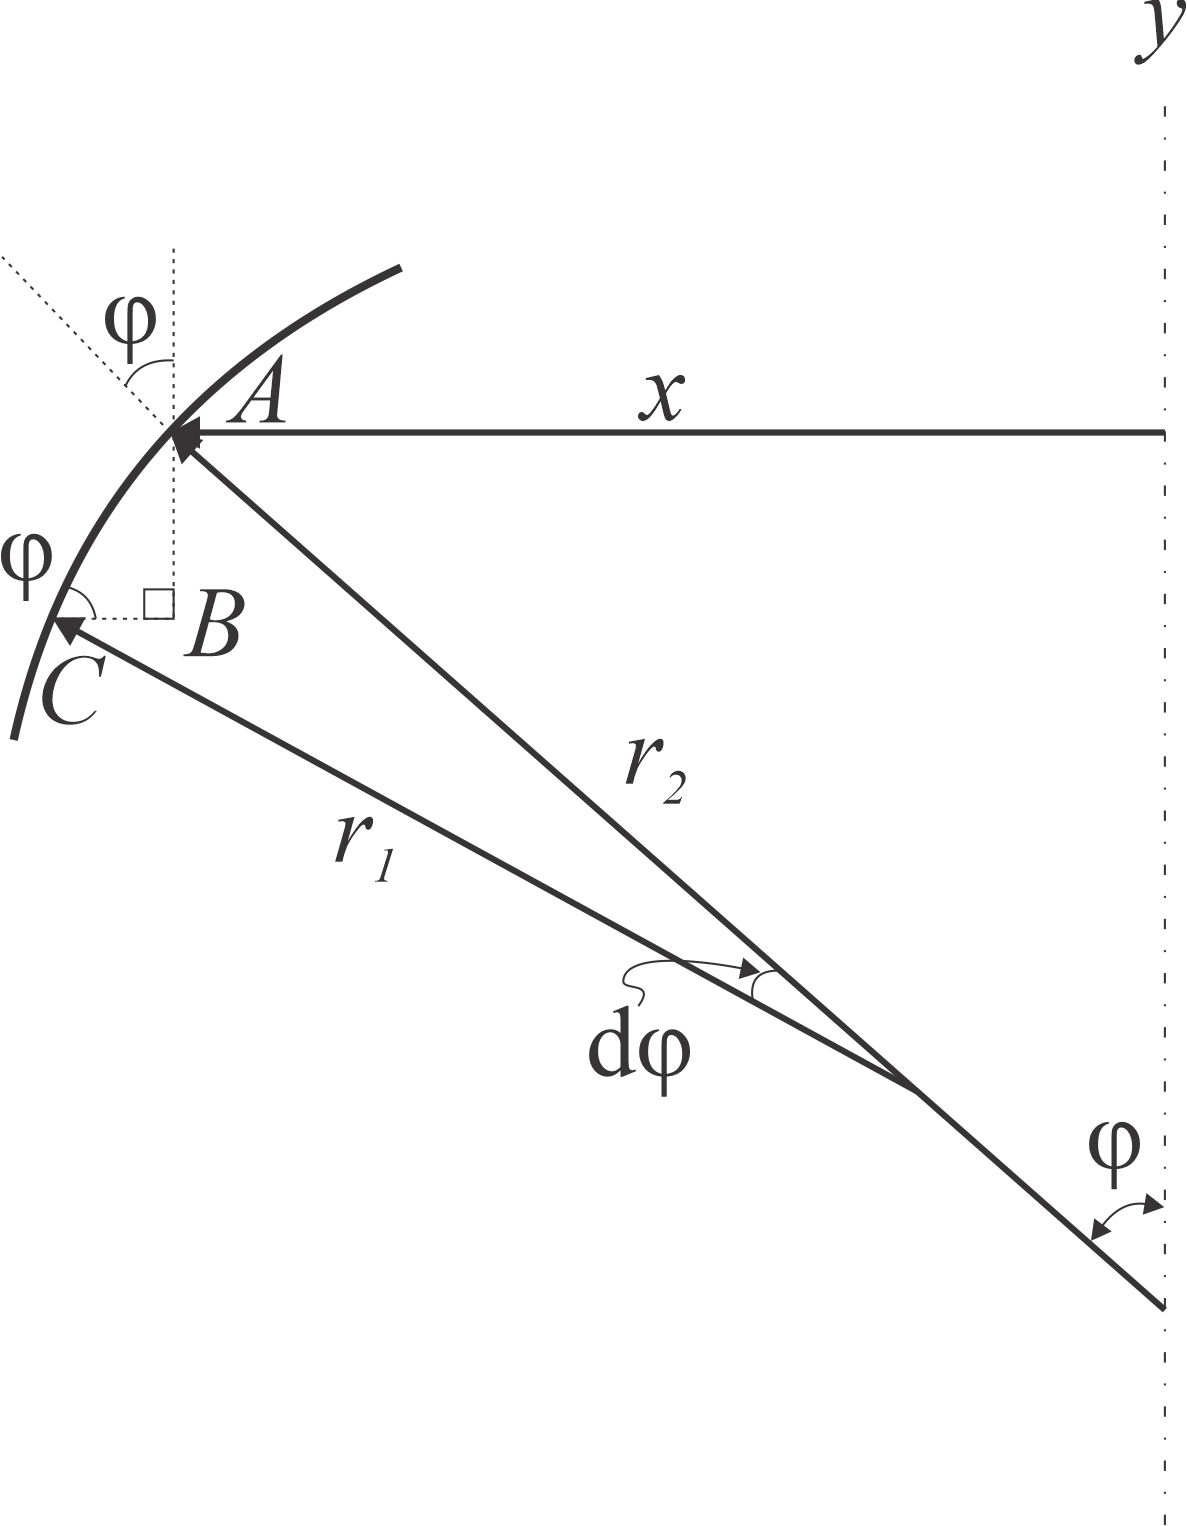
\includegraphics[width=0.5\textwidth]{fig11_19.jpg}
	\caption{Problem 11.20 figure.}
	\label{fig:p11_2}
\end{figure}

Using the figure from Problem 11.20 (figure \ref{fig:p11_2}) and changing variables, in triangle $ABC$ we have $\tan(\phi) = dy/dx$. Replacing the left-hand side of \ref{eq:dy} with $\tan(\phi)$ gives 

\begin{equation}
	\tan(\phi) = \frac{-bx}{a \sqrt{a^2 - x^2}}
	\label{eq:tan_phi}
\end{equation}

whereby solving \ref{eq:tan_phi}

\begin{equation}
	x = \pm \frac{\tan(\phi) a^2}{\sqrt{a^2 \tan^2(\phi) + b^2}} = \pm \frac{\sin(\phi) a^2}{\sqrt{a^2 \sin^2(\phi) + b^2 \cos^2(\phi)}}  
	\label{eq:R1x}
\end{equation}

By substituting $x$ from \ref{eq:R1x} in \ref{eq:dy}

\begin{equation}
	y = \pm \frac{b}{a} \sqrt{a^2 - \frac{\tan^2(\phi) a^4}{a^2 \tan^2(\phi) + b^2}} = \pm b^2 \frac{\cos(\phi)}{\sqrt{a^2 \sin^2(\phi) + b^2 \cos^2(\phi)}}
	\label{eq:R1y}
\end{equation}

Since, in the following, we alway have an even power (squared) of $x$ and $y$, the positives values of both $x$ and $y$ will be used in the following. Now by replacing $x$ and $y$ from \ref{eq:R1x} and \ref{eq:R1y} in \ref{eq:R1}

\begin{equation}
\begin{aligned}
	R_1 =& \frac{(a^4 y^2 + b^4 x^2) \sqrt{a^4 y^2 + b^4 x^2}}{a^4 b^4} \\
	=& \dfrac{\dfrac{a^4 b^4 \cos^2(\phi)}{a^2 \sin^2(\phi) + b^2 \cos^2(\phi)} + \dfrac{b^4 a^4 \sin^2(\phi)}{a^2 \sin^2(\phi) + b^2 \cos^2(\phi)}}{a^4 b^4} \\
	=& \dfrac{a^2 b^2}{{(a^2 \sin^2(\phi) + b^2 \cos^2(\phi)})^\frac{3}{2}}
	\label{eq:R1_1}
\end{aligned}
\end{equation}

Also, we know

\begin{equation}
	\tan(\phi) = \frac{x}{h} = y'(x) = \frac{b^2}{a^2} \frac{x}{y} \Rightarrow h = \frac{a^2}{b^2}y
\end{equation}

From Pythagorem theorem, 

\begin{equation}
\begin{aligned}
	R_2^2 =& x^2 + h^2 = x^2 + \frac{a^4}{b^4} y^2  \\
	=& \frac{a^4 \sin^2(\phi)}{a^2 \sin^2(\phi) + b^2 \cos^2(\phi)} + \frac{a^4}{b^4} \frac{a^4 \cos^2(\phi)}{a^2 \sin^2(\phi) + b^2 \cos^2(\phi)} \\
	=& \frac{a^4}{a^2 \sin^2(\phi) + b^2 \cos^2(\phi)}
	\label{eq:R2}
\end{aligned}
\end{equation}


\end{document}